\section{Is the Cast Operator used?}
\label{sec:casts:stats}

\newcommand{\nproject}{195}
\newcommand{\nloc}{19,264,590}
\newcommand{\nmethod}{1,492,490}
\newcommand{\nmethodwithcast}{99,018}
\newcommand{\nexpr}{57,292,018}
\newcommand{\nCastExpr}{21,491}

\newcommand{\castpercentage}{5.47}

To answer \ref{casts:rq1} (\emph{\crqA}),
we need the following elements:

\textbf{Source Code Analysis.}
We have gathered cast usage using the \ql{} query language.
\ql{} is ``a declarative, object-oriented logic programming language for querying complex, potentially recursive data structures encoded in a relational data model''~\citep{avgustinovQLObjectorientedQueries2016}.
\ql{} allows us to analyze programs at the source code level.
\ql{} extracts the code sources of a project into a Datalog model.
Besides providing structural data for programs, \ie{}, ASTs, \ql{} has the ability to query static types and perform data-flow analysis.
To run our \ql{} queries, we have used the service provided by Semmle.\footnote{\url{https://lgtm.com/}} 

\textbf{Projects.} 
As a code base representative of the ``real world'',
we have chosen open-source projects hosted in \github{},
the world's most popular source code management repository.
To answer \ref{casts:rq1}, we have analyzed \nproject{} \java{} projects in \lgtm{}.

Ultimately, we want to know how many cast instances are used in a given project.
To this end, we gather the following statistics using \ql{}.
We show them here to give an estimation of the size of the code base being analyzed.
The query to gather these statistics is available online.\footnote{\url{https://gitlab.com/acuarica/java-cast-queries/blob/master/ql/stats.ql}}

\begin{center}
\begin{tabular}{lr}
	\hline
	Number of Projects & \nproject \\
	Number of LOC & \nloc{} \\
	Number of Methods & \nmethod \\
	Number of Methods \emph{w/}Cast & \nmethodwithcast \\
    Number of Expressions & \nexpr \\
    Number of Cast Expressions & \nCastExpr \\
	\hline
\end{tabular}
\end{center}

The \emph{Number of Methods} and \emph{Number of Methods w/Cast} values includes only methods with a body, \ie{}, not abstract, nor native.
The \emph{Number of Expressions} value shows how many expressions there are in the ASTs of all source code analyzed.
Finally, the \emph{Number of Cast Expressions} value indicates how many cast expressions (subtype of \code{Expr} as defined by \ql{}) were found.

For our study, we are interested in both upcasts and downcasts.
Thus, we \emph{exclude} primitive conversions in our study
(Sections~$5.1.2$, $5.1.3$, $5.1.4$, and $5.1.13$ from the \java{} Language Specification%
\footnote{\url{https://docs.oracle.com/javase/specs/jls/se7/html/jls-5.html}}
).
The \emph{Number of Casts} value shown above include only reference conversions.
Primitive conversions are always safe (in terms of throwing \code{ClassCastException}.
A primitive conversion happens when both the type of the expression to be casted to and
the type to cast to are primitive types.
Note that with this definition, we include in our study \emph{boxed} types.
Since boxed types are reference types (and therefore not necessarily safe)
we want to include them in our analysis.

We want to know how many cast instances there are across projects.
Thus, we have computed the ratio between methods containing
at least a cast over total number of methods --- with implementation --- in a given project.
The following chart shows this ratio for all analyzed projects:

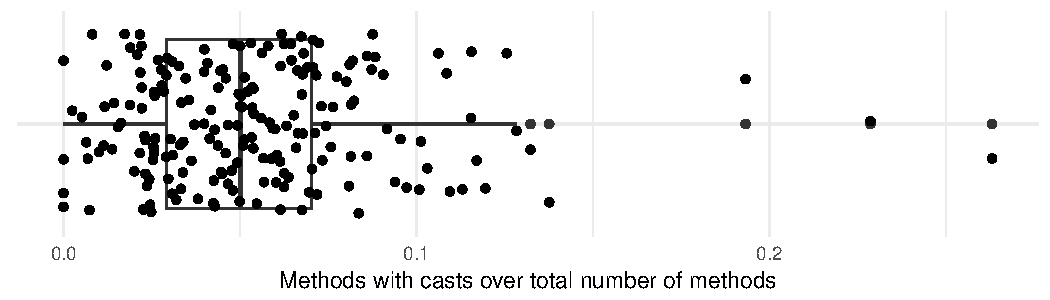
\includegraphics[width=0.9\columnwidth]{analysis/stats-methodwcastXproject.pdf}

All projects have less than 10\% of methods with at least a cast.
Overall, around a \castpercentage{}\% of methods contain at least one cast operation. 
This means there is a low density of casts.
Given the fact that generics were introduced \java{} 5, this can explain this low density.

Nevertheless, casts are still used.
We want to understand why there are casts instances (\ref{casts:rq2}) and how often the use cases that leads to casts are used (\ref{casts:rq3}).
The following sections give an answer to these questions.
